
\section{层流预混火焰}
\subsection{概述}
\subsection{物理描述}
\subsubsection{定义}
\textbf{火焰}是一个以亚音速、自维持传播的局部燃烧区域。
\begin{itemize}
    \item 火焰是局部的,即火焰在任何时候都只占可燃混合物的很小部分;
    \item 亚音速:
    \begin{itemize}
        \item 音速传播的不连续的燃烧波称为\textbf{缓燃波};
        \item 超音速的燃烧波称为\textbf{爆震波}。
    \end{itemize}
\end{itemize}

\subsubsection{重要特征}
随着火焰移动的观察者可以感受到未燃的混合物以一定的速度向其流动,这个速度就是火焰传播速度\(S_\mathrm{L}\)。
\begin{equation}
    \rho_\mathrm{u} S_\mathrm{L} A \equiv \rho_\mathrm{u} v_\mathrm{u}A = \rho_\mathrm{b} v_\mathrm{b}A
\end{equation}
可以把火焰分成两个区域:
\begin{itemize}
    \item \textbf{预热区}几乎没有热量释放出来
    \item \textbf{反应区}释放出大量的化学能。火焰厚度一般在常压下只有毫米级,反应区可以进一步划分为:
    \begin{itemize}
        \item 快速反应区:极窄、双分子反应,常压下典型厚度小于一毫米,梯度很大。
        \item 慢速反应区:三个自由基的合成反应,范围可以延伸到几毫米。
    \end{itemize}
\end{itemize}

\subsubsection{典型的实验室火焰}
\begin{figure}[H]
    \centering
    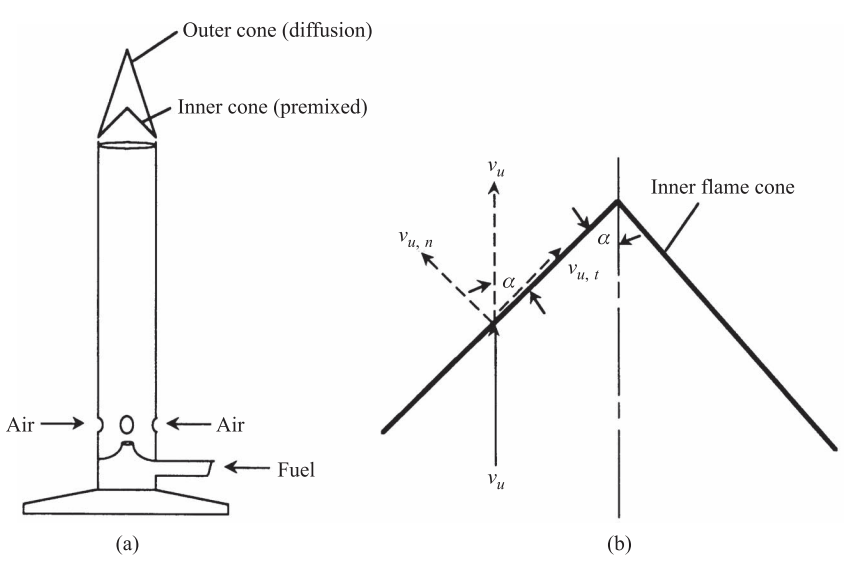
\includegraphics[width=.32\textwidth]{img/bunsen.png}
\end{figure}
由于火焰传播速度和未燃气流速度在火焰面法线方向的分量处处相等:
\begin{equation}
    S_\mathrm{L} = v_\mathrm{u}\sin \alpha
\end{equation}

\subsection{简化分析}
\subsubsection{假设}
\begin{enumerate}
    \item 一维、等面积、稳态流
    \item 忽略动能、势能,忽略黏性力做功,忽略热辐射。
    \item 忽略火焰前后的很小的压力变化,即压力是常数。
    \item 热扩散和质量扩散分别服从傅里叶定律和菲克扩散定律。假定是二元扩散。
    \item  路易斯数,\(Le = \alpha/\mathcal{D} = k/(\rho c_p \mathcal{D})\)为1。
    \item 混合物的比热容与温度及其组成无关。
    \item 燃料和氧化剂通过一步放热反应生成产物。
    \item 氧化剂等于化学当量或者过量混合,燃料完全消耗。
\end{enumerate}

\subsubsection{守恒定律}
\begin{enumerate}
    \item 质量守恒;
    \item 组分守恒,利用总包反应方程式,根据燃料的流量,分别表达燃料、氧化剂和产物三者的守恒方程;
    \item 能量方程:利用Shvab-Zeldovich形式的能量守恒方程,总和利用\(Le=1.0\)的假设,得到方程。
\end{enumerate}

\subsubsection{求解}
假定温度是\_/\(^-\)的形式,即温度在很小的距离\(\delta\)内,从低温到了高温,定义这个距离为火焰厚度。后面就代入到方程里面开始积分吧。主要处理的方程就是:
\begin{equation}
    {\dot{m}}^{\prime\prime}{\frac{\mathrm{d}T}{\mathrm{d}x}}-{\frac{1}{c_{p}}}{\frac{\mathrm{d}\left(k{\frac{\mathrm{d}T}{\mathrm{d}x}}\right)}{\mathrm{d}x}}=-{\frac{{\dot{m}}_{F}^{\prime\prime\prime}\Delta h_{c}}{c_{p}}}.
\end{equation}
一共积分两次,一次从\(-\infty\to\infty\),一次从\(-\infty\to\delta/2\)

定义平均反应速度为:

\begin{equation}
    \overline{\dot{m}}_\mathrm{F}''' = \frac{1}{T_\mathrm{b} - T_\mathrm{u}}\int_{T_\mathrm{u}}^{T_\mathrm{b}}\dot{m}_F'''\dd T
\end{equation}
实际计算的时候,也采用下面的方法:
\begin{equation}
    \overline{\dot{m}}_F''' = \overline{\dot{\omega}}_F MW_\mathrm{F}
\end{equation}
计算\(\overline{\dot{\omega}}_F\)的时候,用平均的温度和浓度就好。

注意,由于我们在推导的过程中是在\(-\infty\to \delta/2\)这一区间上进行积分的,其中包含了一个假设就是认为\(\dot{m}_\mathrm{F}'''\)等于0,所以我们在计算平均温度时:
\begin{equation}
    \overline{T} = \frac{1}{2}\left[\frac{1}{2}(T_\mathrm{b} + T_\mathrm{u})+T_\mathrm{b}\right]
\end{equation}

最后的结果是:
\begin{equation}
    S_\mathrm{L} = \left[-2\alpha (\nu+1)\frac{\overline{\dot{m}}'''_\mathrm{F}}{\rho_\mathrm{u}}\right]^{1/2}
\end{equation}

\begin{equation}
    \delta = \left[\frac{-2\rho_\mathrm{u}\alpha}{(\nu+1)\overline{\dot{m}}_F'''}\right]^{1/2}
\end{equation}
或者也可以写作:
\begin{equation}
    \delta = 2\alpha/S_L
\end{equation}

\subsection{详细分析}
\subsection{影响火焰速度和厚度的因素}
\begin{enumerate}
    \item 过量空气系数:稍稍缺氧时\((phi>1)\),火焰传播速度最大,那个时候往往火焰厚度最薄;
    \item 燃料化学结构;
    \begin{enumerate}
        \item 烷烃最大火焰传播速度为(0.7 m/s),几乎与烷烃的碳数无关;
        \item 非饱和碳氢化合物,碳原子少的火焰传播速度大;
        \item 但是碳原子多到一定程度也就基本不下降了。
    \end{enumerate}
    \item 未燃气体温度:提高未燃气体温度可以大大促进化学反应速度,从而增大\(S_L\)的值;
    \item 压力的影响:不是说\(n\)等于2的时候就没有影响了,实际上,这个时候时成反比;
    \[{\cal S}_{L}\propto\overline{{{T}}}^{0.375}T_{u}T_{b}^{-n/2}\exp(-E_{A}/2R_{u}T_{b})P^{(n-2)/2}\]
\end{enumerate}

\subsection{选定燃料的火焰传播速度计算式}
Metghalhi-Kech关系式:
\begin{equation}
    S_\mathrm{L} = S_\mathrm{L,ref}\left(\frac{T_\mathrm{u}}{T_\mathrm{u,ref}}\right)^\gamma\left(\frac{P}{P_\mathrm{ref}}\right)^\beta (1-2.1 Y_\mathrm{dil})
\end{equation}
具体细节可以看237页。

\subsection{熄火、可燃性、点火}

\subsubsection{冷壁熄火}
\textbf{点火和熄火准则}:
\begin{enumerate}
    \item 仅当足够多的能量加入到可燃气体中,使和稳定传播的层流火焰一样厚的一层气体的\textbf{温度升高到绝热燃烧温度},才能点燃。
    \item 板形区域内化学反应的放热速率必需近似平衡于由于热传导从这个区域散热的速率。
\end{enumerate}

考虑一个间距为\(d\)的平行板,研究它的熄火问题。热量流失依靠导热:
\begin{equation}
    \left|\frac{\dd T}{\dd x}\right| = \frac{T_\mathrm{b} - T_\mathrm{w}}{d/b}
\end{equation}

这里的\(b\)显然是一个至少比2大的数字,而且实际上大不少。后面经过数学上的一番倒腾,可以得到:
\begin{equation}
    d = \sqrt{b}\delta
\end{equation}

不难发现,熄火距离是要比火焰厚度要大的。

\subsubsection{可燃极限}

\textbf{可燃下限}是允许稳态火焰传播的燃料含量最低的混合气体(\(\Phi<1\)),而\textbf{可燃上限}则指允许火焰传播的燃料含量最高的混合气体(\(\Phi>1\))。

\subsubsection{点火}

着火分类:
\begin{enumerate}
    \item 化学自燃:不需外界加热,靠自身化学反应就可着火;
    \item 热自燃:混合气加热到一定温度在整个容积中着火。
\end{enumerate}

\textbf{简化的点火分析}:
\begin{itemize}
    \item 确定临界半径;
    \item 确定最小点火能量。
\end{itemize}

这里也是利用傅立叶导热定律进行分析,结论是:
\begin{eqnarray}
    R_\mathrm{crit}&=& (\sqrt{6}/2)\delta\\
    E_{\mathrm{ign}}&=&61.6P\left(\frac{c_{p}}{R_{b}}\right)\left(\frac{T_{b}-T_{u}}{T_{b}}\right)\left(\frac{\alpha}{S_{L}}\right)^{3},
\end{eqnarray}其中\(R_b = R_u/MW_b\)。

\textbf{压力、温度和当量比的影响}
\begin{equation}
    E_\mathrm{ign}\propto P^{-2}
\end{equation}
增大压力或者初始温度,最小点火能量都会降低。

\subsubsection{火焰稳定}
\textbf{回火}:火焰进入燃烧器和喷口内继续传播而不熄灭;发生在燃料气流减小或关闭时。危害:损坏燃烧设备,甚至爆炸。回火通常是瞬态的,发生在燃料气流减小或关闭时。局部火焰传播速度超过局部气流速度。当燃料气流停止时,火焰就会通过任何比熄火距离大的管子或喷口而发生回火。所以说火焰传播速度大的燃料比较容易发生回火,In comparison with 人工煤气 and 甲烷,后者回火稳定性更加好。

\textbf{推举}:火焰与燃烧器管子或喷口不接触,而是稳定在离喷口一定距离的位置;容易形成未燃气体逃逸。
